\section{Applications of community
detection}\label{applications-of-community-detection}

The extensive work behind developing and validating methods for
community detection is presumably meant to work toward a goal of using
community detection for some concrete applications. In this area, the
field shows its (young) age---it is somewhat difficult to find published
examples where the methods have been applied to solve a specific problem
or gain significant new insight into a system. Below, I discuss some of
the examples that do exist in the research literature, in the fields of
\protect\hyperlink{social-network-analysis}{social network analysis},
\protect\hyperlink{networks-of-scholarship}{networks of scholarship},
\protect\hyperlink{biological-networks}{biological networks}, and
\protect\hyperlink{other-research}{others}. Besides published research,
I speculate on the (mostly unpublished) applications of community
detection outside of academia, and present an example of using community
detection in the context of a small data science project to address a
question of interest.

\hypertarget{social-network-analysis}{\subsection{Social network
analysis}\label{social-network-analysis}}

Social networks often contain intuitive and potentially interesting
community organization, so it is not surprising that there has been
interest in applying community detection to various forms of social
data. The enormous popularity of online social network platforms like
Facebook and Twitter have made detailed social network data available at
a massive scale. These data are not available equally to
everybody---most popular social networking applications are proprietary
and much of their data are reserved for internal research. It is likely
that these companies are using community detection to explore patterns
in their data, but not publishing all of their results.

One published study of Facebook was conducted by Traud et al.
\autocite{traud_social_2012}. They examined the Facebook friend network
from 100 American colleges and universities (at the time of this study,
Facebook was restricted to these institutions). They performed community
detection using several modularity-optimizing techniques and compared
the community structure against several (self-reported) categorical
demographic variables---gender, class year, high school, major, and
residence. Fig.~\ref{fig:facebook} shows a visualization of community
structure with class year---the variable most strongly associated with
community structure. The authors find some patterns that we might
reasonably expect, such as class year being associated with friend
communities, and high school being more associated with communities at
larger institutions (where one is more likely to find multiple people
from the same high school). They also identify some patterns that would
be interesting to study further, such as that females were more likely
to have friends within their same residence.

\begin{figure}
\centering
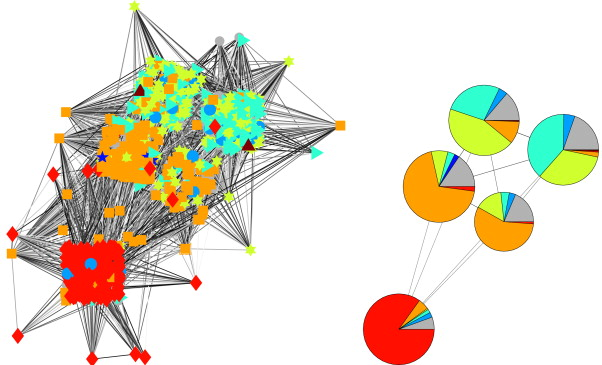
\includegraphics{img/traud2012_fig2_facebook.jpg}
\caption{Community structure from the Reed College Facebook friend
network. On the left, colors and shapes of nodes indicate different
class years. On the right, the communities are condensed into pies. The
size of the pies correspond to the number of nodes, and darker edges
mean more connections between communities. A correlation between class
year and community structure can be seen. Figure from
\autocite{traud_social_2012}.}\label{fig:facebook}
\end{figure}

\begin{figure}
\centering
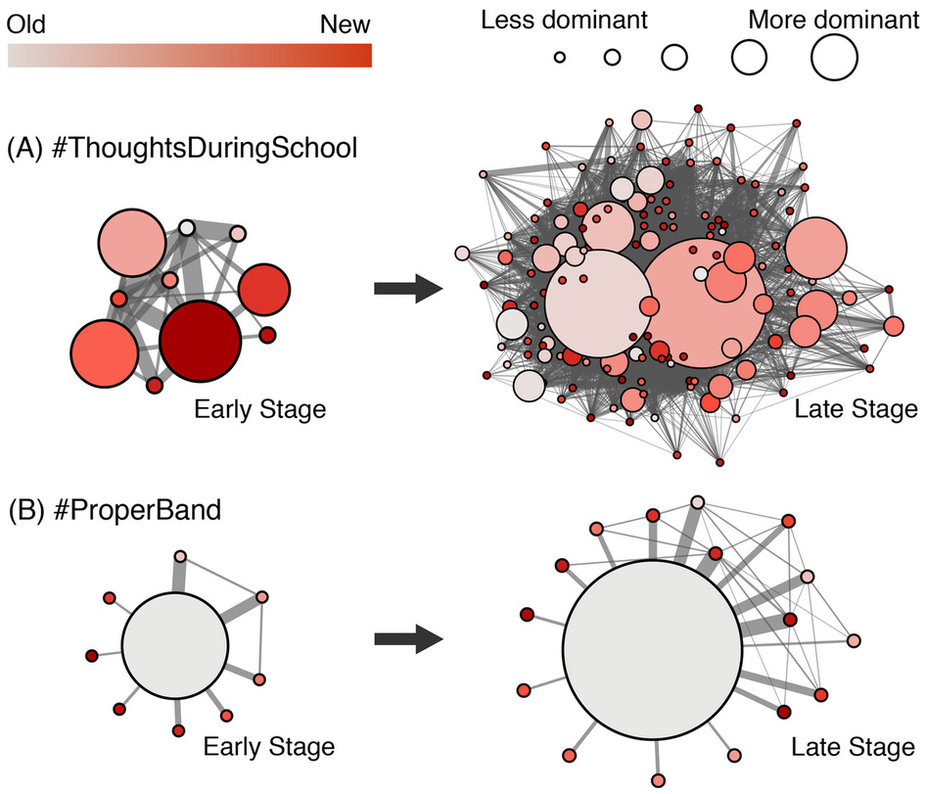
\includegraphics{img/weng2013_fig4_viraltwitter.jpg}
\caption{The evolution of a viral meme (A) vs.~a non-viral meme (B).
Each node is a community, with size proportional to the number of tweets
produced by the community, and color indicating the relative time that
the hashtag was first used by the community. Figure from
\autocite{weng_virality_2013}.}\label{fig:viraltwitter}
\end{figure}

Weng et al. \autocite{weng_virality_2013} used community detection to
study the virality of memes on Twitter. Since the question of interest
was one of information flow, they used Infomap, a flow-based community
detection method (see subsection
``\protect\hyperlink{the-dynamical-perspective}{The dynamical
perspective}'' in section
``\protect\hyperlink{community-detection-methods}{Community detection
methods}'' above). They identified communities in networks of
reciprocal-follower relationships among Twitter users.
Fig.~\ref{fig:viraltwitter} shows the evolution of a viral meme vs.~a
non-viral meme (here a meme corresponds to a hashtag), with the
communities represented as nodes. The results suggest that a meme that
is less concentrated in one community is more likely to spread, and that
community structure might be helpful in predicting the virality of
memes. They go on to apply a random forest classifier for new memes that
takes into account community features, and find that these features are
helpful in predicting whether a meme will go viral.

\hypertarget{networks-of-scholarship}{\subsection{Networks of
scholarship}\label{networks-of-scholarship}}

The collective human endeavor of knowledge generation and organization
can be represented as a directed network of scholarly publications with
citations between them. The citation links between publications can been
viewed as a proxy for influence or information flow. De Solla Price
recognized the potential of this representation in the mid 20th century
\autocite{de_solla_price_networks_1965}, and over the years much work
has been done in this meta-scientific research area, which has been
given terms such as ``bibliometrics,'' ``scientometrics,'' and ``science
of science''. In these networks, publications (or journals, or authors)
form communities, which intuitively represent different fields of
scholarship. Rosvall and Bergstrom \autocite{rosvall_maps_2008} applied
the \protect\hyperlink{the-dynamical-perspective}{Infomap} algorithm on
the journal citation network to build a map of science, visualizing
information flows between disciplines (see fig.~\ref{fig:journals}).
Rosvall and Bergstrom also applied community detection at different time
points to build maps of how science changes over time, revealing the
formation of the standalone field of neuroscience by 2007 from various
other disciplines starting in 2001, shown in Fig.~\ref{fig:alluvial}
\autocite{rosvall_mapping_2010}. Communities in citation networks have
also been used in a recommendation system for scholarly articles
\autocite{west_recommendation_2016}; and as a way of representing
distance between scientific fields, in combination with other measures
of distance such as language barriers arising from the use of jargon
\autocite{vilhena_finding_2014}.

\begin{figure}
\centering
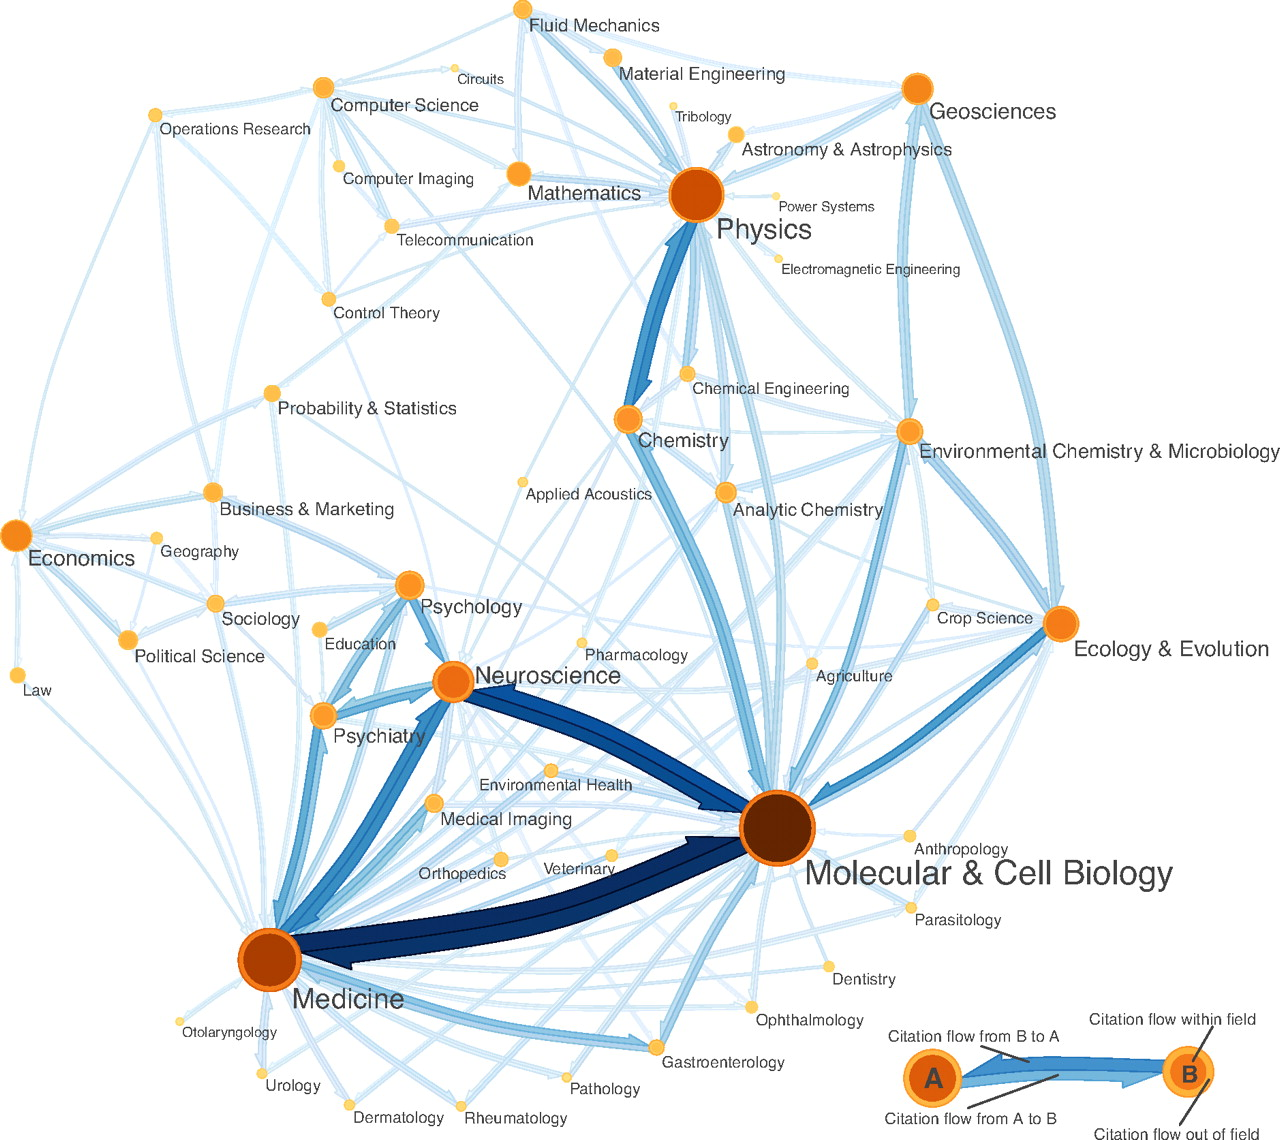
\includegraphics{img/rosvall2008_fig3_journals.jpg}
\caption{A map of science based on a journal citation network of
articles published in 2004, and citations to articles published in the
previous 5 years.. Nodes represent communities found using the Infomap
algorithm; they are hand-labeled according to the research topic of the
journals they contain. The size of the nodes reflects the fraction of
time a random walker spends within each community, and directed and
weighted links between nodes represent citation flow between
communities. We can see a ``U'' shaped pattern, with social sciences and
engineering at opposite ends and medicine, molecular biology, and
physics forming the bridge. Figure from
\autocite{rosvall_maps_2008}}\label{fig:journals}
\end{figure}

\begin{figure}
\centering
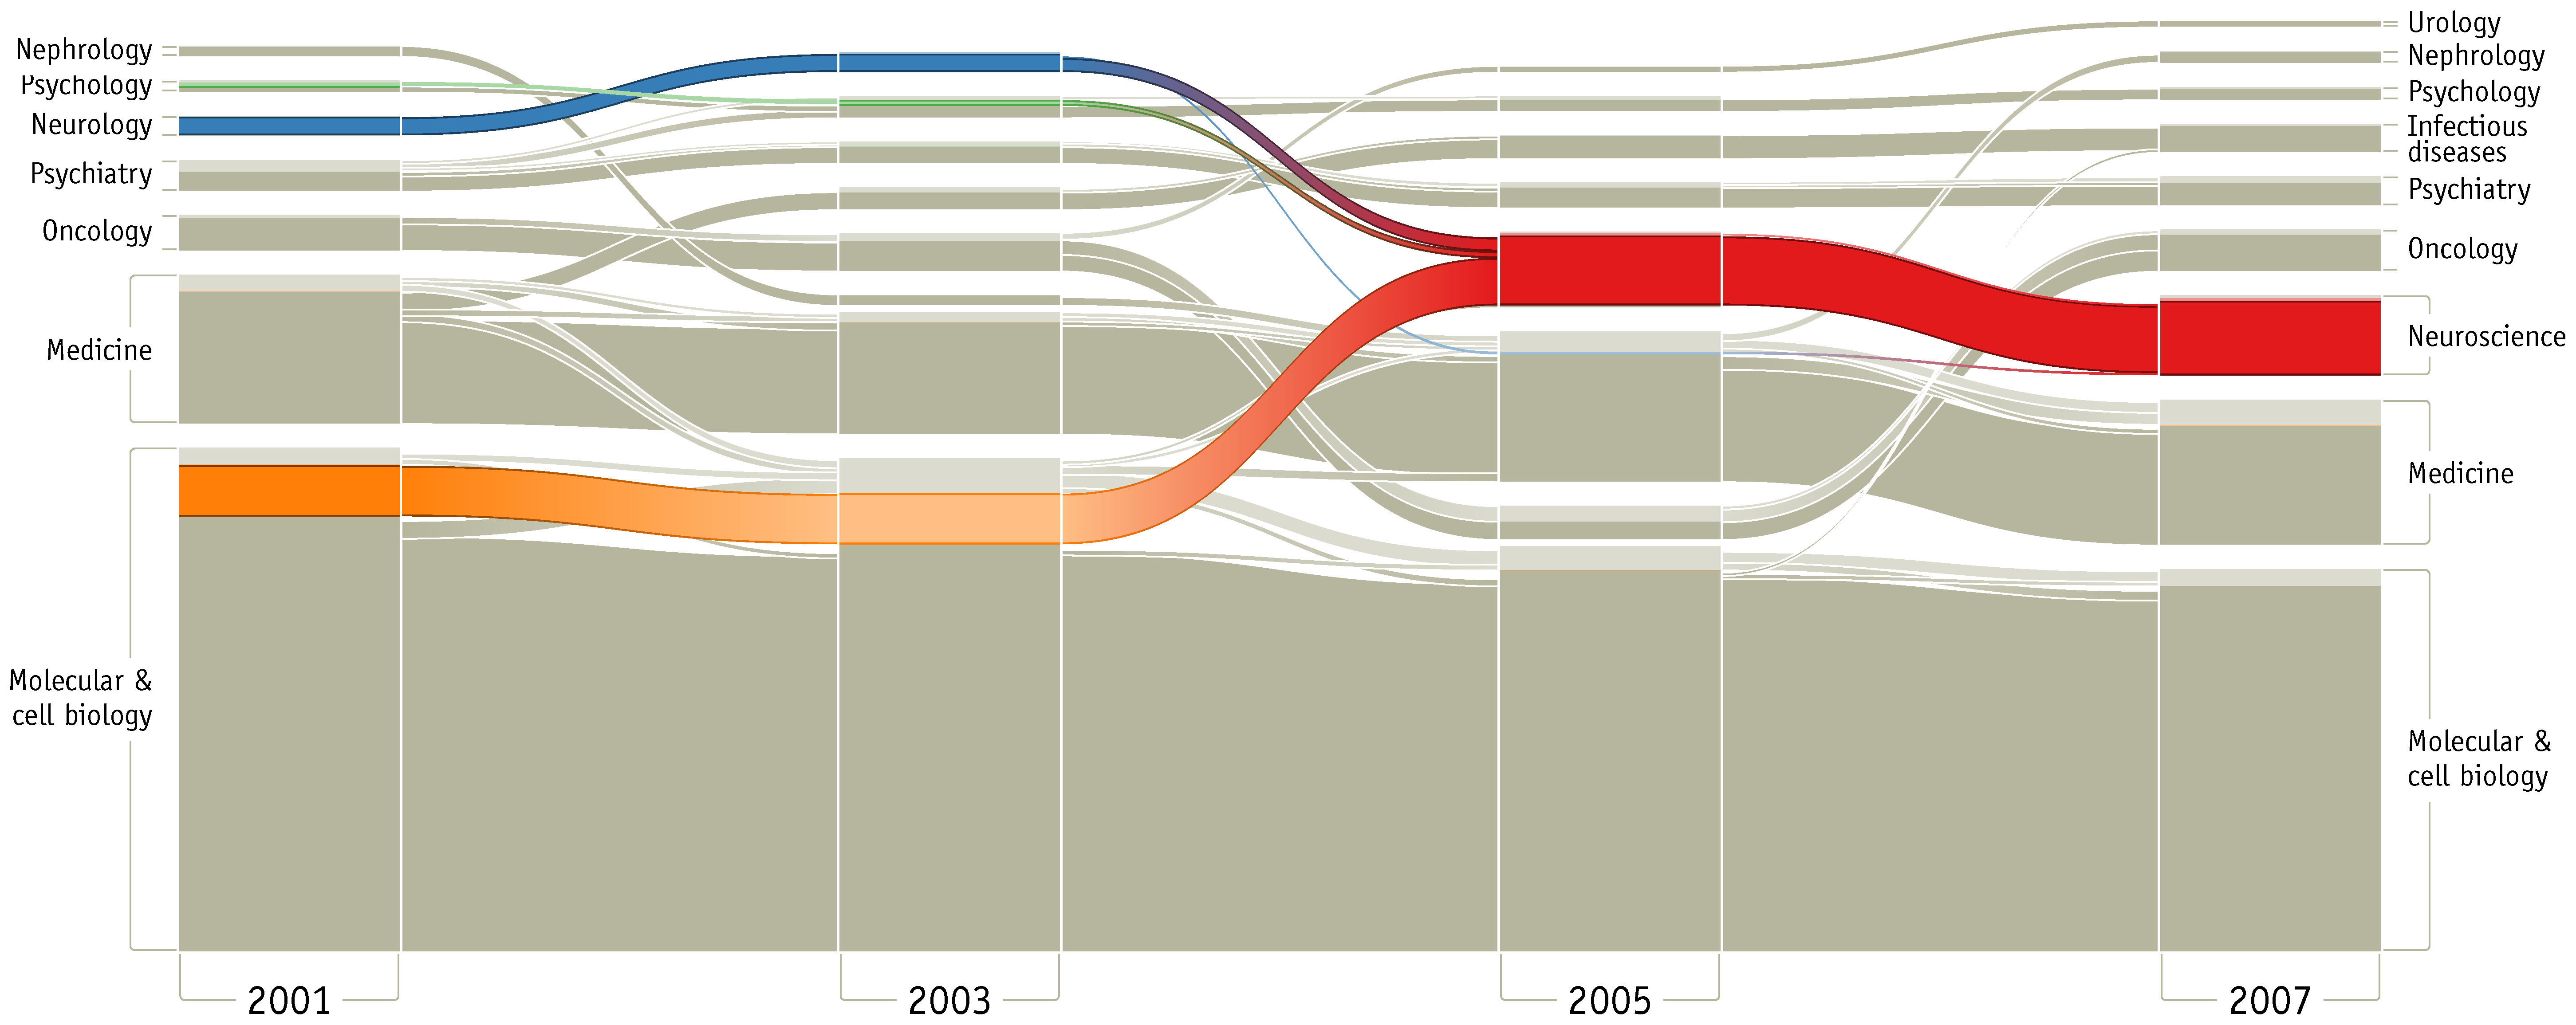
\includegraphics{img/rosvall2010_fig3_alluvial.png}
\caption{Alluvial diagram of scientific disciplines changing over time,
identified by detecting communities in the journal citation network
using Infomap. All journals that appear as neuroscience by 2007 are
highlighted to show how that field emerged from parts of other
disciplines. Figure from
\autocite{rosvall_mapping_2010}}\label{fig:alluvial}
\end{figure}

\hypertarget{biological-networks}{\subsection{Biological
networks}\label{biological-networks}}

Many biological systems can be thought of as structured interactions
between functional elements, often with (possibly hierarchical) modular
structure. It is natural to think of these systems as networks, and to
see promise in the prospect of identifying communities in this network
representation.

Protein-protein interaction networks are constructed from data collected
in experiments that identify molecular interactions between proteins.
Community detection on these networks, for example using the
Girvan-Newman edge betweenness method, has been shown to be effective in
identifying what are known as ``functional modules'' in these
networks---groups of proteins that interact in the service of a
particular cellular process. Clusters found in these networks correspond
to existing annotations, suggesting promise for the automated analysis
of experiments. These methods were also found to be robust against false
positive interactions, which is important considering that experimental
results can contain considerable noise \autocite{dunn_use_2005}. Chen
and Yuan \autocite{chen_detecting_2006} integrated multiple protein
interaction datasets containing hundreds of microarray expression
profiles for \emph{Saccharomyces cerevisiae} (brewer's yeast) to form a
weighted graph, in which the weights correspond to dissimilarity between
genes' expression profiles. By classifying the genes into functional
modules using a modified version of the Girvan-Newman method, they were
able to predict the function of the as-yet not annotated yeast gene
\emph{YLR419w} to be chromosome segregation.

Another biological network that has been studied is the directed network
of neuronal connections---the ``connectome''. Dynamically-minded
community detection methods (see subsection
``\protect\hyperlink{the-dynamical-perspective}{The dynamical
perspective}'' in section
``\protect\hyperlink{community-detection-methods}{Community detection
methods}'' above) are especially relevant for these networks as the
connectome represents a system of information flow, which is what these
methods model. Bacik et al. \autocite{bacik_flow-based_2016} grouped the
neurons of \emph{C. elegans} using flow-based methods. These detected
communities showed good agreement with previous understanding of
functional neuronal groups. They were then able to perform \emph{in
silico} ablations of neurons---computer simulations in which they
removed nodes and looked at the resulting disruption on community
structure. By doing this, they identified neurons important to the
network flow, and presumably important to the neuronal function of the
organism. These included neurons known to be important, as well as
previously uninvestigated neurons that can be candidates for future
study.

\hypertarget{other-research}{\subsection{Other examples in the research
literature}\label{other-research}}

Zhang et al. \autocite{zhang_community_2008} analyzed Congressional
cosponsorship networks in the United States Congress in order to study
partisan polarization. They created a two-mode (bipartite) network
between legislators and legislation, and then projected this network to
a one-mode (unipartite) network in which nodes are legislators, and
links between legislators represent the fact that they have cosponsored
bills together. They then compared the optimal modularity of these
networks at different time points with the observed modularity using
party affiliation as community membership. In other words, they were
interested in how close the structural communities seen in the network
were to the ``communities'' of political party. They found that the
difference between these two values decreased over time (1979--2004),
indicating that the cosponsorship behavior of legislators was
increasingly aligning with party affiliation---i.e., that polarization
was increasing.

Lupu and Traag \autocite{lupu_trading_2013} used community detection to
study the impact of trade networks among nations on the potential for
conflict between nations. States that trade with each other are known to
have less conflict with each other. The authors argue for extending this
to trade communities. Two states may also see a reduced risk of conflict
even if they do not have a strong trade relationship, if they are
indirectly linked by trade. The authors test this theory by applying the
Louvain modularity-optimizing community detection algorithm on a network
of trade flows between states. They find that states in the same trade
community are significantly less likely to experience conflict with each
other, even controlling for direct trade relationships.

\subsection{Non-research applications}\label{non-research-applications}

Besides the published examples of applications of community detection,
there are likely many that have not been published, either due to
secrecy around industry or state knowledge, or simply because the people
involved are not oriented toward academic publishing. One such area is
marketing: community information on various types of consumer networks
could be useful for targeted marketing
\autocite{labatut_detection_2012}. This is also related to
recommendation systems, as discussed in the context of scholarly
publications above; graph clustering approaches to recommendation have
appeared in the published literature
\autocites{reddy_graph_2002}{fouss_random-walk_2007}, and it is probable
that more exists unpublished. Another likely use for community detection
is in the identification of criminal or terrorist organizations, and
while the potential for this is evident in the literature
\autocites{krebs_mapping_2002}{nath_crime_2006}{carlos_andre_community_2012}{clauset_developmental_2012}{waskiewicz_friend_2012}{ferrara_detecting_2014},
it is likely that the successes seen from following such approaches
would not be made public.

Finally, it possible that community detection methods have become
another part of the data analysis toolkit, in a way that its direct
applications may often be part of the routine practice of data
scientists (a term not reserved for academic scientists) and not
published as research. As an example, I direct the reader to the section
\protect\hyperlink{visualization}{``Visualizing community structure in
networks''} below, in which I use community detection to help answer a
question of interest: Which research labs are actively working on
research related to visualizing group structure in networks?
